
 \documentclass{article}
\usepackage{graphicx}
\graphicspath{ {./images/} }
\usepackage{float}
% Required for inserting images

\title{CSC111 Project Report: A Reinforcement Learning Approach to Connect 4}
\author{Elsie Chan, Annie Tan, York Hay Ng}
\date{\today}

\begin{document}

\maketitle

\section{Introduction}

\par Our project aims to develop an AI model that can play Connect 4 through Q-learning and effectively compete against human players.

Connect 4 is a two-player strategy game where players take turns placing coloured tokens into a 7 by 6 grid. The tokens fall vertically to the lowest possible space in any given column. The objective of Connect 4 is to be the first to form a horizontal, vertical, or diagonal line using 4 of their own coloured tokens. For the purposes of our project, we will shrink the board size to 5 by 5 and add an additional way to win: when a player’s coloured tokens form a wrap-around horizontal line in the grid.

Q-learning is a type of model-free reinforcement learning algorithm that operates by learning the value of an action at a particular state. The algorithm maintains a Q-table that contains the expected quality or reward of all possible action-state pairs. The agent then selects the action that maximise its expected reward over time. Through training the agent, the agent will learn to select actions that maximise its expected reward, resulting in an optimised algorithm for decision-making. [1]

To calculate the Q-value in a given state $S_{t}$ applying an action $a_{t}$, ie $Q_{new}(S_{t},a_{t})$, we must first define $\alpha$ - the learning rate, which determines how strongly a new Q-value would affect the existing value, and $\gamma$ - discount, which depicts the extent of importance of immediate reward $r_{t}$ over future rewards. The action $a_{t}$ with the highest Q-value is the optimal action. [1]

$$Q_{new}(S_{t},a_{t}) = (1 - \alpha)Q(S_{t},a_{t}) + \alpha(r_{t} + \gamma max_{a}Q(S_{t+1},a))$$

According to the TA's feedback, we decided to focus more on incorporating a tree-based approach to our Q-learning models using a game tree. Based on the feedback, Monte Carlo tree search was suggested, however, due to time constraints, we were unable to accommodate this recommendation. The feedback also suggested implementing minimax algorithm, but the minimax algorithm may not be suitable for our tree-based project.

We chose this project goal as we were inspired by CSC111’s Assignment 2. We want to use the concept of a game tree to develop a more comprehensive AI for playing a mathematical game. Connect 4 is a strategic yet relatively complex game, and therefore, developing an AI model that can play Connect 4 would involve understanding the game’s rules and potential strategies.

Additionally, we believe that this could be a fun and engaging project to see if we can develop an AI model that could challenge human players.

In conclusion, the project question that we want to answer is:

\textbf{How can we use Q-learning to train an AI model that plays Connect 4 with a decent performance, especially compared to human players?}


\section{Datasets: AI Models}

There are 4 datasets in this project, which are different GameTree instances depicting different AI models.

\begin{enumerate}
    \item 5x5\_tree\_randagent\_P1\_demo
    \item 5x5\_tree\_randagent\_P1
    \item 5x5\_tree\_randagent\_P2
    \item 5x5\_tree\_rand+ai\_P2
\end{enumerate}

They are all generated in the ai\_training module described in the next section. Note that they are binary files generated by pickle.dump(). They can be formatted back to GameTree instances with pickle.load().


\section{Computational Overview}

The ConnectFour class, within the connect\_four module, is responsible for handling the game state of each Connect Four game instance. It stores the current game board in a numpy 2-dimensional array, with zeros representing empty slots, 1 representing player 1's tokens and 2 representing player 2's tokens. Additionally, the attribute possible\_moves stores the "legal" moves that players can make as a list of tuple coordinates. The board is updated with the record\_move method, which makes a move at the specified location corresponding to whose turn it is, while updating possible\_moves. The method get\_winner determines if any player has won the game, by checking every row, column and diagonal (using numpy's ndarray.diagonal method) if there are four consecutive tokens in the board.

\bigskip

The players module defines the Player classes that will interact with the ConnectFour game instance, making moves in the game with the make\_move method. Human players can play and interact via the HumanPlayer class, which makes moves in the board according to the player's specified locations. The player that AIPlayer instances will be trained against, RandomAgent, makes moves randomly from the list of ConnectFour.possible\_moves. 

The AI player, AIPlayer, aims to make moves ``intelligently''. When it is initialized, it sets self.complete\_tree to be the given game tree, or to an empty GameTree if no binary file including a GameTree instance is given. AIPlayer makes a move by traversing down the GameTree to the corresponding game state, keeping track of the current position in the tree with the attribute self.curr\_tree. From the possible moves in GameTree.\_subtrees, it picks the move with the greatest q\_value (or picks amongst the moves with the greatest q\_values) as dictated by GameTree.q\_values. If self.curr\_tree no longer contains a GameTree or a leaf node is reached, therefore representing a situation where the AIPlayer can no longer pick moves from the GameTree, it will randomly pick a move from the list of legal moves in ConnectFour.possible\_moves.

If AIPlayer is being trained, instead of setting self.curr\_tree to None whenever it can't pick any more moves from the GameTree, it will expand the current GameTree by adding new subtrees with the move it picks. The explore\_rate also defines the chance at which the AIPlayer will explore new moves despite being able to pick moves from the current GameTree.

The play\_against method in AIPlayer allows us to train AIPlayer by developing a game tree and updating the q\_values for the moves in the GameTree, through simulating any number of games between AIPlayer and an arbitrary opponent Player, where the exploration rate decreases linearly across the defined range. The method also allows for analysing the performance of the AIPlayer without training it.

\bigskip

In the GameTree that the AIPlayer traverses, the nodes are represented by q\_values, which is a dictionary storing all the possible "legal" moves from the given game\_instance, mapped to the q-value associated with that move. The subtrees are stored in the \_subtrees attribute, containing a dictionary of tuples of moves from the list of possible moves mapped to the GameTree after that move has been played in game\_instance.

GameTree contains the add\_subtree method, which adds another GameTree to self.\_subtrees and is used in training the AIPlayer. Given an entire move sequence of a game from start to finish, the method update\_q\_tables is responsible for calculating and updating the q-values of those moves in their corresponding GameTree instances. This method is implemented recursively. Starting from the last move in move\_sequence, the q-value of each move is calculated. For the last move that the AIPlayer makes, its q-value is calculated according to the formula outlined in the introduction, applying (when winning) or subtracting (when losing) rewards depending on the outcome of the game. For the rest of the moves, their corresponding q-values is calculated by the same formula but without the granting of immediate rewards. 

\bigskip

The ai\_training module contains several functions which uses AIPlayer.play\_against to train, or demonstrate the performance of the AIPlayer in different scenarios. By running the function run\_games, it will first demonstrate the training of the AIPlayer as player 1 against a RandomAgent as player 2 in 10,000 games. It will then (train and) show the performances of AIPlayer as player 1 or 2 against RandomAgent and another AIPlayer instance in order to show how well AIPlayer plays in this game. If you want to see the performance of the AIs, just run this module in Python console and call run\_games().

\bigskip

The graphplot module has a GraphPlot class that uses the plotly library to handle the visualization of the Connect 4 game results via graphs. The dashboard consists of three plots:

\begin{enumerate}
    \item A scatter plot showing the outcome of each game, where 1 represents a win for player 1, 2 represents a win for player 2, and 0 represents a draw. 
    \item A scatter plot showing the cumulative win percentage for player 1 over all games played, and hovering over each point in the graph reveals the cumulative win percentage at that point in time.
    \item A bar chart showing the number of wins and draws for player 1 and player 2, and hovering over each bar in the chart reveals the exact number of wins or draws for that player.
\end{enumerate}

Overall, the GraphPlot class provides an interactive way to analyse the performance of the AI agents in the Connect 4 game.

\bigskip
pygame is used to provide a graphical user interface for the Connect 4 game. The GameInterface class initializes the pygame screen and uses pygame.draw.circle and pygame.draw.rect to create a Connect Four game board and tokens in draw\_board(). Additionally, pygame allows us to handle different event types. Specifically, the runner() function in main.py uses the pygame.event.get() function to get a list of all events that have occurred. If the pygame.QUIT event is detected, the game ends. If a pygame.MOUSEBUTTONDOWN event is detected, i.e. if the human player clicks on a particular column in the game board, then a move is then made and recorded for the current player.


\section{Instructions for running the program}

\begin{enumerate}
    \item Install all required libraries listed under requirements.txt.
    \item Obtain the datasets (ie the trained AI models) from UTSend. Unzip the trained AI models. You should be able to get a directory named ``AI Models'' with binary files inside. Place the directory in the same place as the Python source codes.
    \item Run main.py. A pygame window displaying a 5x5 Connect 4 game board will pop up, and you can choose to drop the tokens into any column of your choosing (Click anywhere in the column that you want to place the token in).
    There will be a prompt for you to choose whether you want to play first or second, and key in either 1 or 2. Once the choice is made, the game will begin, with the chosen player dropping their first token into the board. The AI player will then take its turn and drop a token into the board as well. The game will continue until either a player wins or a draw is reached. When the game ends, the program will display the winner or indicate if the game ended in a draw.
    \begin{figure}[h]
        \centering
        \includegraphics[scale=0.4]{images/starting.png}
        \par Initial pygame window
    \end{figure}
    \begin{figure}[h]
        \centering
        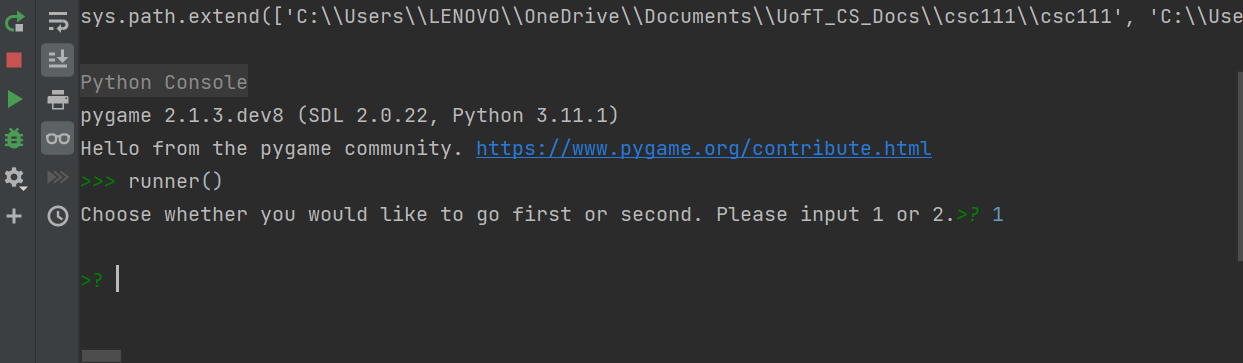
\includegraphics[scale=0.5]{images/input.png}
        \par Key in either 1 or 2 here
    \end{figure}
    \begin{figure}[H]
        \centering
        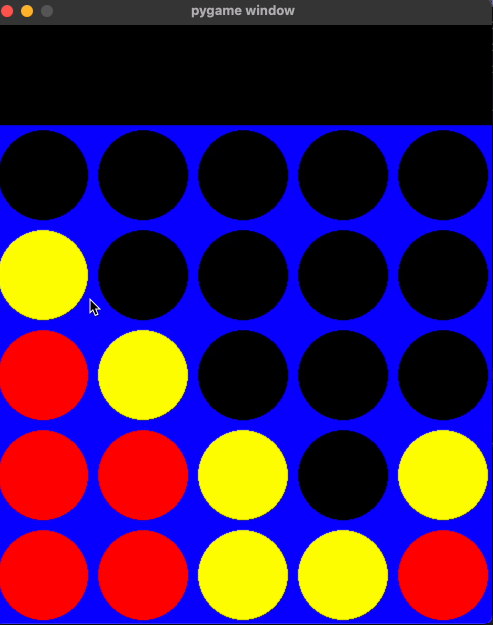
\includegraphics[scale=0.6]{images/output.png}
        \par Sample game board at the end of the game
    \end{figure}
    \begin{figure}[H]
        \centering
        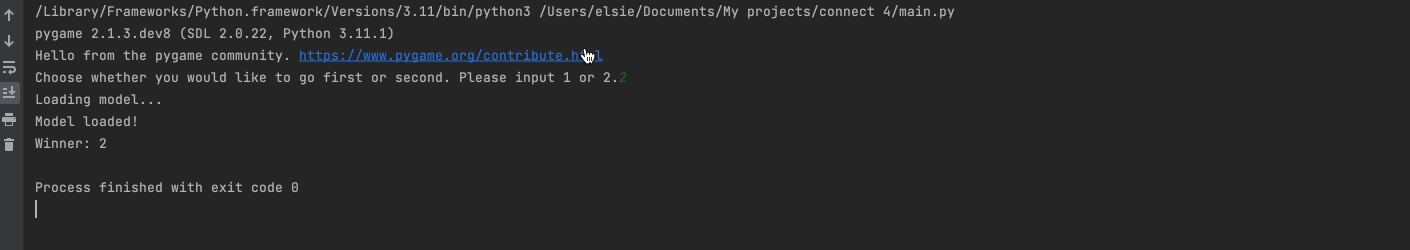
\includegraphics[scale=0.5]{images/output2.png}
        \par Sample output of winner
    \end{figure}
\end{enumerate}

Remarks: If you want to see the performances of the AI against different Player instances, you can run the ai\_training module in Python console and call run\_games() in it.

\section{Changes to project plan}

Instead of using the standard 6x7 Connect 4 game board size, we shrank it to 5x5 in order to reduce the size and complexity of the GameTrees for our AIPlayers. Moreover, we trained our AI with an agent which makes entirely random moves instead of being able to predict one step ahead. Also, we just created a normal instead of an animated graph for showing the performance between players so that it is more efficient in training AIPlayer instances and showing game results. 

\section{Discussion}

To analyze and interpret the results of our program, we compared the performance of a trained player against that of a random player.

\subsection{Trained P1 vs Random P2}

When comparing a trained player 1 (P1) against a random player 2 (P2), the results showed that the trained P1 outperformed the random P2.

According to Figure 1, when training P1 under 100000 games, the cumulative win percentage for P1 is around 0.6-0.7, and P1 won 0.68 of the games. 

\begin{figure}[h]
    \centering    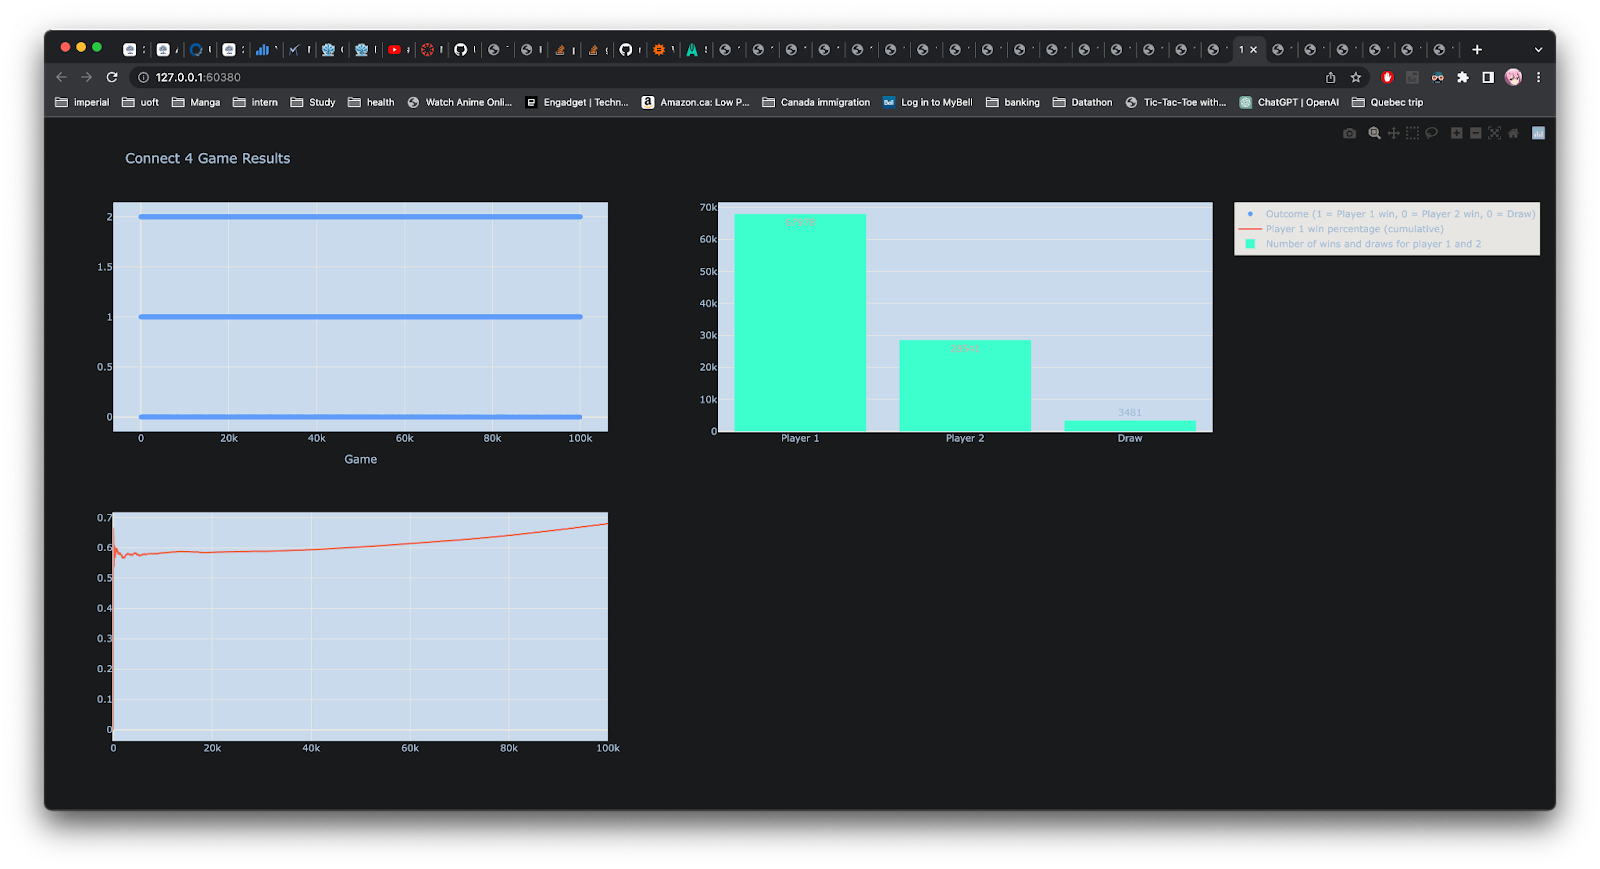
\includegraphics[scale=0.24]{images/1.png}
    \caption{Results of training P1 under 100,000 games}
    \label{fig:my_label}
\end{figure}

According to Figure 2, when comparing the performance of a trained P1 against a random P2 for 1000 games, the cumulative win percentage for P1 improved to about 0.89.

\begin{figure}[H]
    \centering   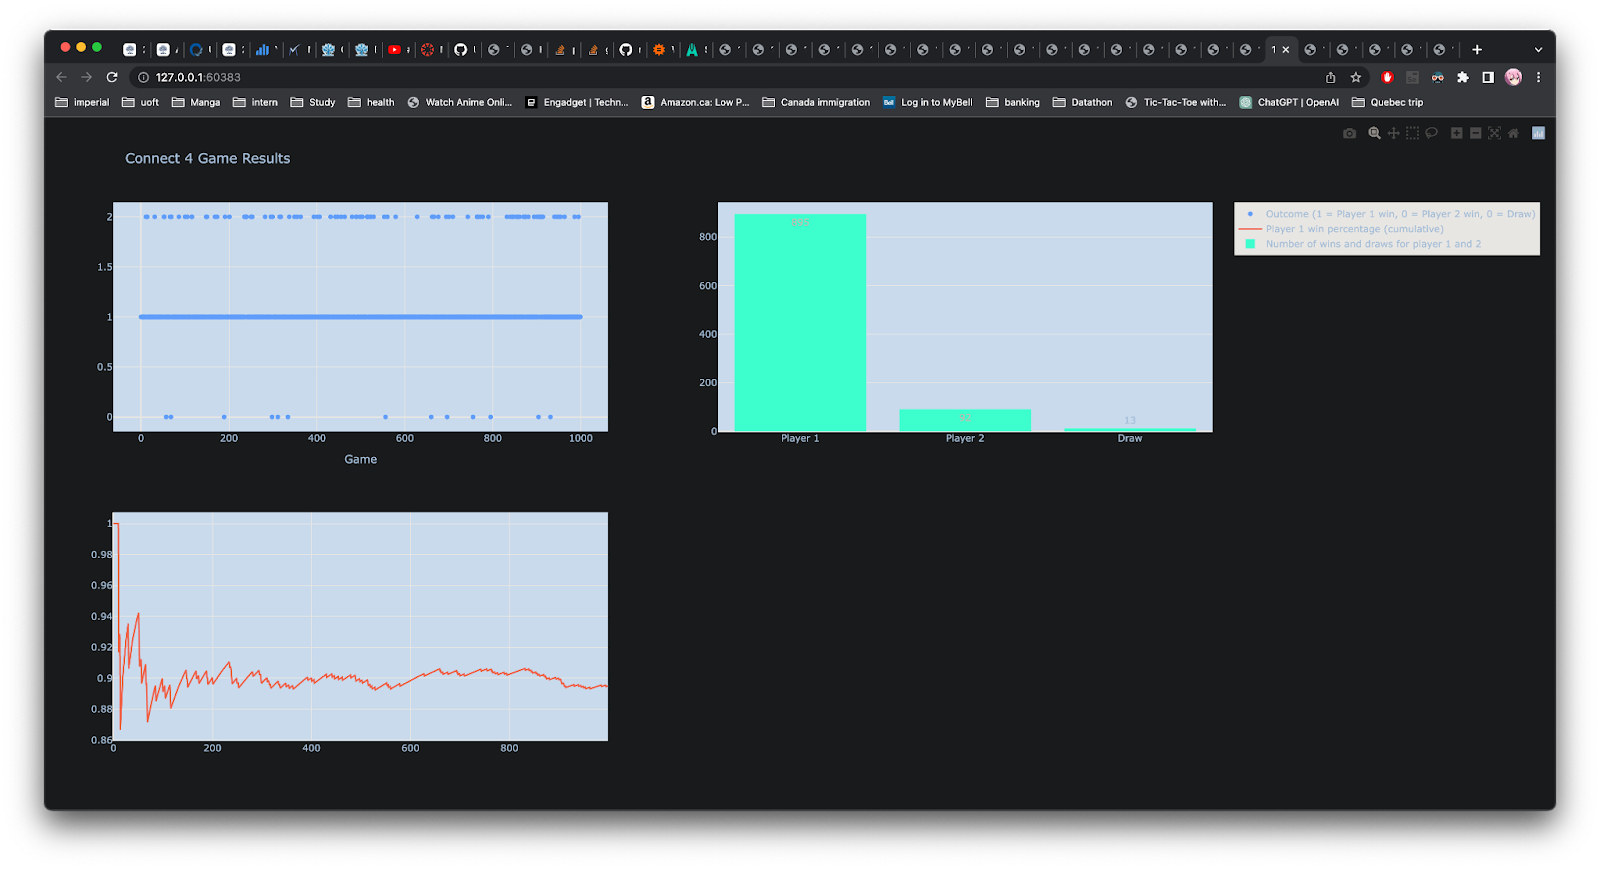
\includegraphics[scale=0.24]{images/2.png}
    \caption{Performance results of trained P1 against random P2 in 1,000 games}
    \label{fig:my_label}
\end{figure}

\subsection{Random P1 vs Trained P2}

When comparing a random P1 against a trained P2, the results showed that the trained P2 outperformed random P1.

According to Figure 3, when training P2 under 200000 games, the cumulative win percentage for P2 is around 0.47. 

\begin{figure}[H]
    \centering
    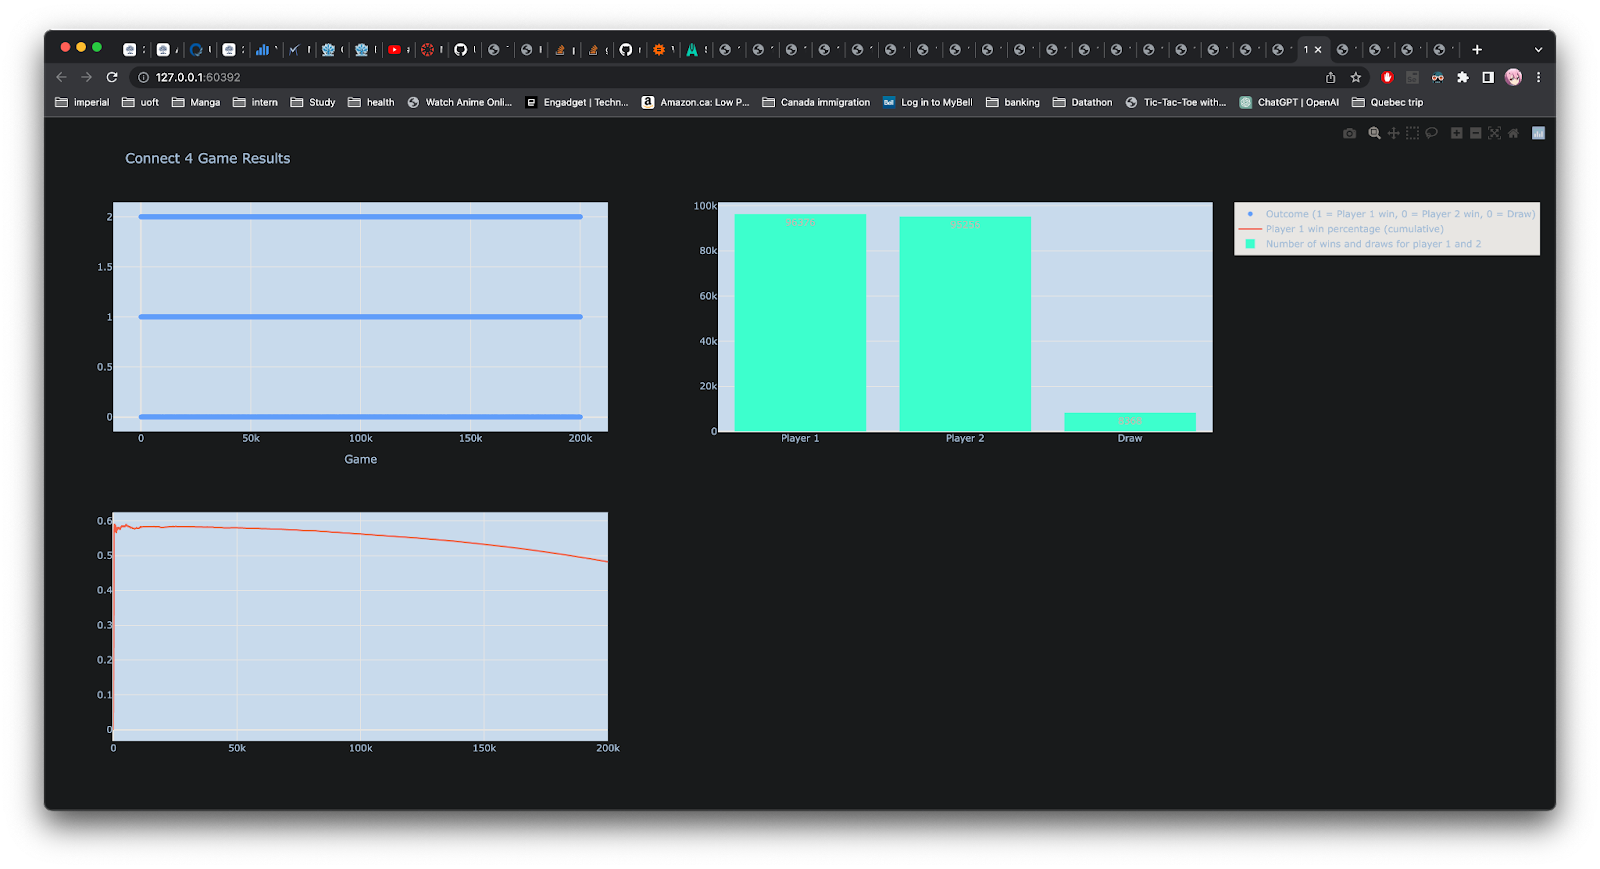
\includegraphics[scale=0.24]{images/3.png}
    \caption{Results of training P2 under 200000 games}
    \label{fig:my_label}
\end{figure}

Additionally, according to Figure 4, when comparing the performance of a trained P2 against a random P1 under 1000 games, the cumulative win percentage of the random P1 was around 0.25, which means that the cumulative win percentage of trained P2 is about 0.73 (the rest 0.02 is draw).

\begin{figure}[h]
    \centering
    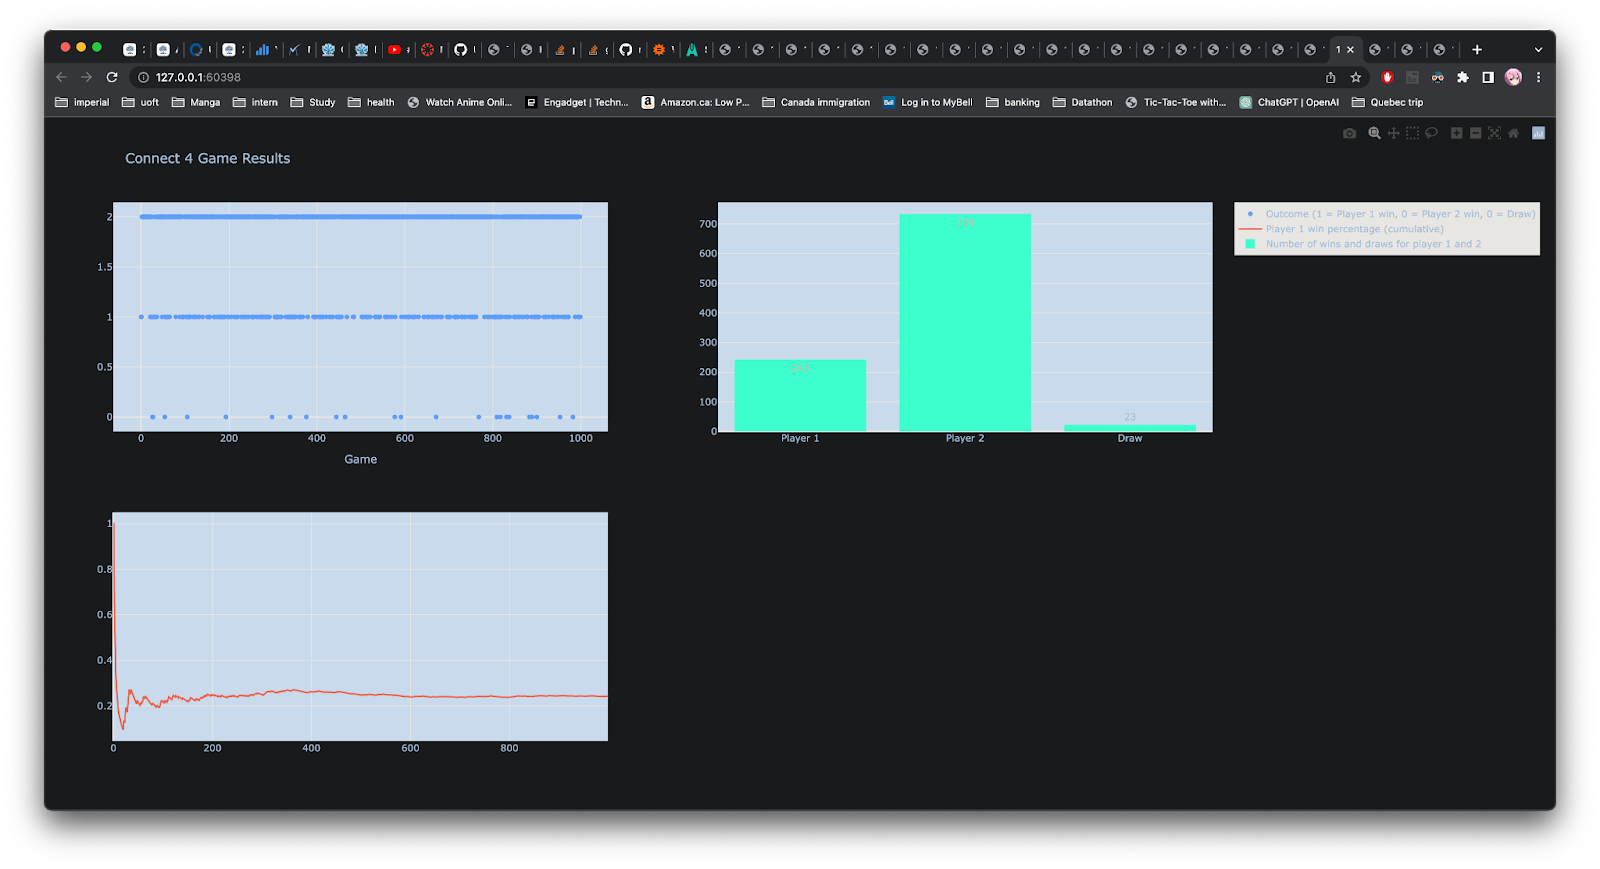
\includegraphics[scale=0.24]{images/4.png}
    \caption{Results of performance of trained P2 against random P1 in 1000 games}
    \label{fig:my_label}
\end{figure}

While the results clearly show that trained players fare better than random players, we now investigate the question of how trained players fare against other trained players. 

\subsection{Trained P1 vs Trained P2}

When comparing trained player 1 and trained player 2 under 1000 games, according to Figure 5, trained P1 won 0.51 of games, and trained P2 won 0.40 of games (the rest 0.11 is draw). Therefore, although P2 was trained under twice the number of games as P1, trained P1 performs slightly better than P2.

\begin{figure}[h]
    \centering
    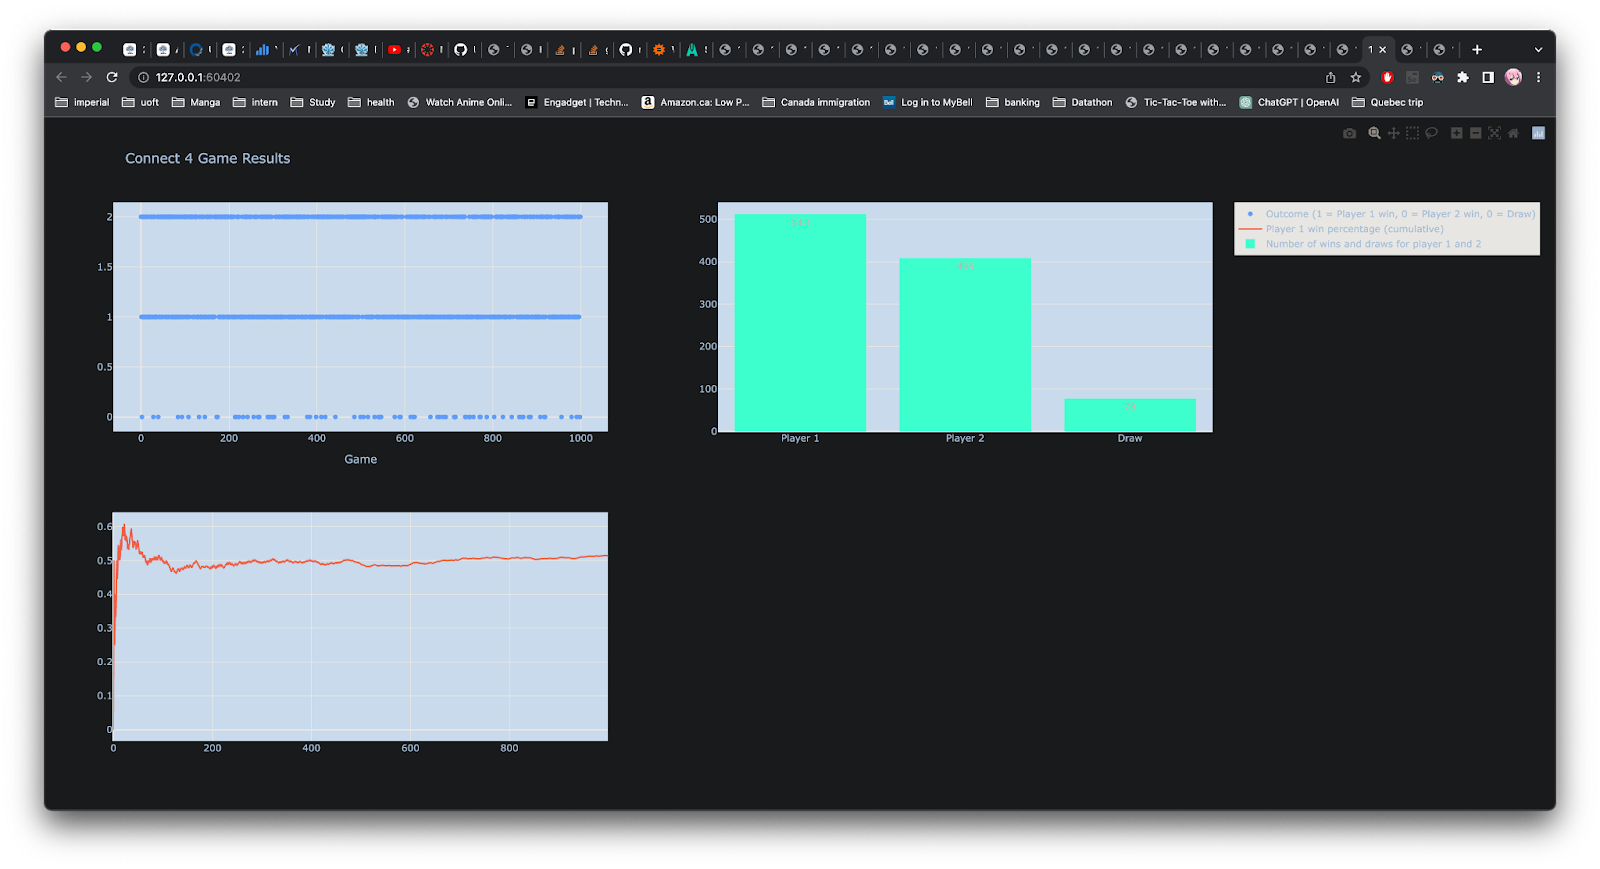
\includegraphics[scale=0.24]{images/5.png}
    \caption{Results of performance of trained P1 against trained P2 in 1000 games}
    \label{fig:my_label}
\end{figure}

\subsection{Trained P1 vs Retrained P2}

Now, we compare the performance of trained P1 against retrained P2.
During the retraining of P2, according to Figure 6, trained P1 won 0.57 of all games, and P2 won 0.41 of all games. 

When comparing the performance of trained P1 against retrained P2, according to Figure 7, the cumulative win percentage of trained P1 is 0 throughout all 1000 games, and that the retrained P2 won all 1000 games. 

\begin{figure}[H]
    \centering
    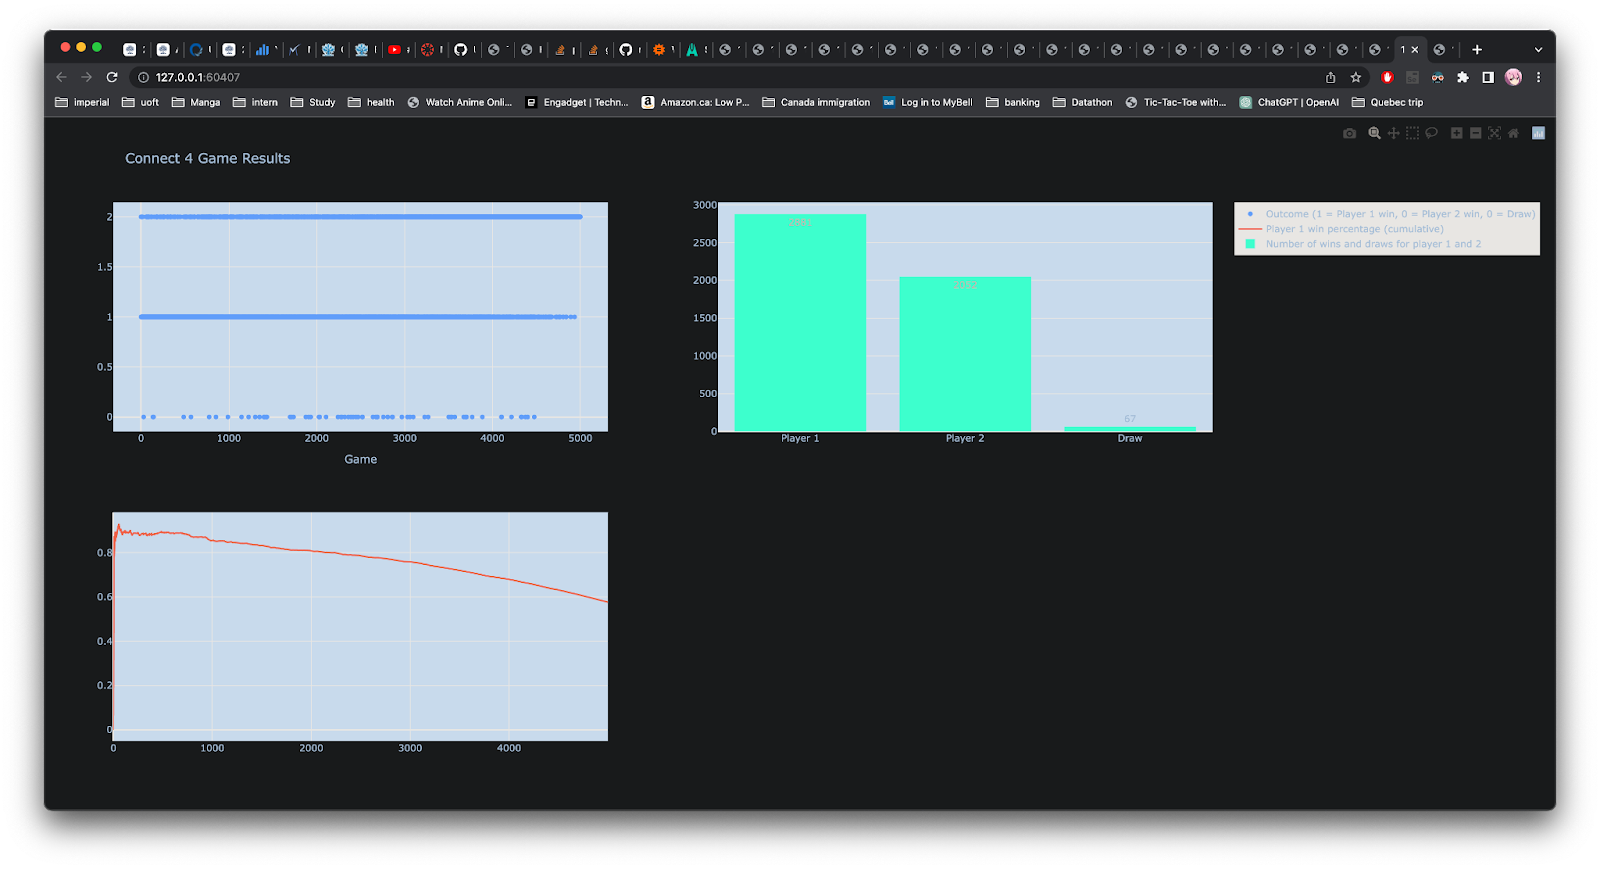
\includegraphics[scale=0.24]{images/6.png}
    \caption{Results of retraining P2 in 5000 games}
    \label{fig:my_label}
\end{figure}

\begin{figure}[H]
    \centering
    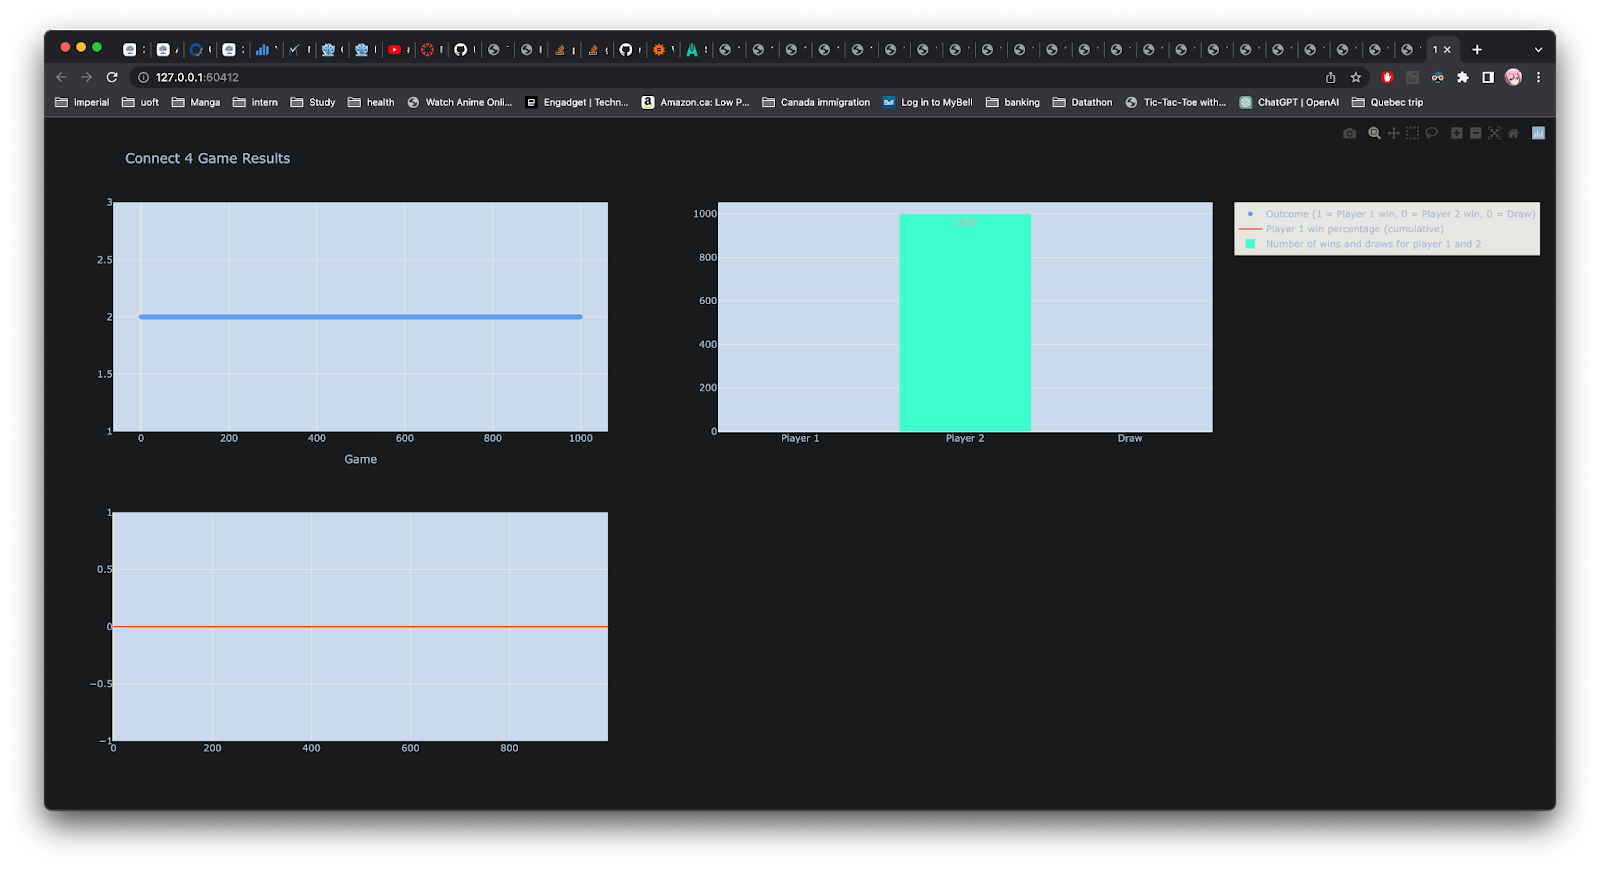
\includegraphics[scale=0.24]{images/7.png}
    \caption{Results of performance of trained P1 against retrained P2 in 1000 games}
    \label{fig:my_label}
\end{figure}

\subsection{Analysis and Conclusion}

It is notable that while P2 was trained on twice as many games as P1, which implies that P2 may have an advantage in terms of exposure to different game situations and strategies. However, when evaluated against random opponents, the performance of trained P1 is better than trained P2, with trained P1 winning 0.89 of all games and trained P2 winning 0.73 of all games.

The more significant difference in performance occurred when P2 was retrained against P1. In this case, the retrained P2 agent won 1.0 of all games, while trained P1 was unable to win any games. This suggests that P2 learnt from its previous experiences and developed a strategy that targeted P1's weaknesses.

Overall, the results demonstrate the importance of training AI agents against different opponents, as well as the potential for AI agents to improve and adapt through retraining.


\section{References}

1) Tic-tac-toe with tabular Q-learning. Nested Software. (2019, July 25). Retrieved March 6, 2023,

from https://nestedsoftware.com/2019/07/25/tic-tac-toe-with-tabular-q-learning-1kdn.139811.html

2) Badr Mario, Liu David, and Bernuy Angela Z. (2023) CSC111 Assignment 2 source code. Retrieved March 6, 2023.

3) Pygame Documentation. Pygame Front Page - pygame v2.1.4 documentation. (n.d.). Retrieved March 7, 2023, from https://www.pygame.org/docs/

4) Plotly. Plotly Python Graphing Library. (n.d.). Retrieved April 2, 2023, from https://plotly.com/python/ 


\end{document}
